
\chapter{Triển khai và đánh giá}
\section{Triển khai}
\subsection{Yêu cầu}
\subsubsection{Kiến thức cơ bản}
\subsubsection{Thư viện bậc cao}
\subsection{Nội quy, hướng dẫn}

\#\#\# Tại sao cần phải viết?

Một trong những vấn đề khi làm việc nhóm là sự hiểu nhau giữa các thành viên trong team.
Mình có thể khăc phục bằng cách trao đổi nhiều hơn. Xác nhận nhiều hơn. Nhưng khi nhóm trở nên lớn.
Thành viên trong nhóm cũng có sự thay đổi liên tục. Hoặc khung giờ làm việc, lịch trình ngày làm việc của mọi người khác nhau. Thì việc này dần trở nên khó khăn hơn. Một chức năng phát triển xong cách khoảng thời gian dài sau đó nâng cấp. Nếu cùng một người thì đây là giao tiếp với chính bản thân mình.

Vậy để giải quyết vân đề này, mọi người cần viết viết và viết. Viết đung là tốn thời gian và làm chậm năng suât của mình. Nhưng đối vơi cac vấn đề trên. Viết là cách giải quyết.

\#\#\# Viết cái gì, viết như thế nào?

Viết bât cứ cái gì có thể viết. Cách thức xác định cái gì cần viết bao gồm:

- Nếu như mình không làm công việc này nữa. Thì chỉ lại cho ai, chỉ những gì. Suy ra viết những gì học được.
- Nếu như ai đó cần giúp mình, thì mình cần chỉ họ đọc gì, hiểu gì để làm. Suy ra viết nhũng gì hiểu được trong từng trường hợp.
- Nếu như ai đó thay đổi công việc mình đã làm, họ cần lưu ý những gì. Suy ra viết những dự định hoặc rủi ro lường trước với công việc mình đang làm.



\subsubsection{Báo cáo kiểm soát công việc}

\#\# Dành cho thay đổi, thêm mới tính năng
\#\#\#\# Thay đổi hoặc thêm mới gì
\#\#\#\# Mô tả hướng thay đổi, li do thay đổi.

\#\# Dành cho sửa lỗi

\#\#\#\# Nguyên nhân
Nguyên nhân gây lỗi.

\#\#\#\# Điều tra
Các thay đổi trong quá khứ gây ra lỗi hoặc điều tra các chức năng liên quan đến thay đổi.
Các hiểu nhầm hoặc yêu cầu thay đổi gây ra lỗi.
Link pull request gây ra lỗi.

\#\#\#\# Hướng thay đổi
Hướng thực hiện thay đổi

\#\# Phạm vi can thiệp
\#\#\#\# Màn hình (page)
\#\#\#\# Nhóm components
\#\#\#\# Schema (ItoaJS)

\#\# Kết quả
Chụp ảnh màn hình, kết quả API

\#\# Lưu ý


\subsection{Quản lí mã nguồn}
\subsubsection{ocopee}
\subsubsection{gateway}
\subsubsection{accounts}
\subsubsection{docs}
\subsubsection{sellers}
\subsubsection{Cài đặt}
\subsubsection{Khởi chạy}
\paragraph{Backend}
%	
\begin{figure}[h]
	\caption{State diagram \cite{web:mongo:why}}
	\centering
	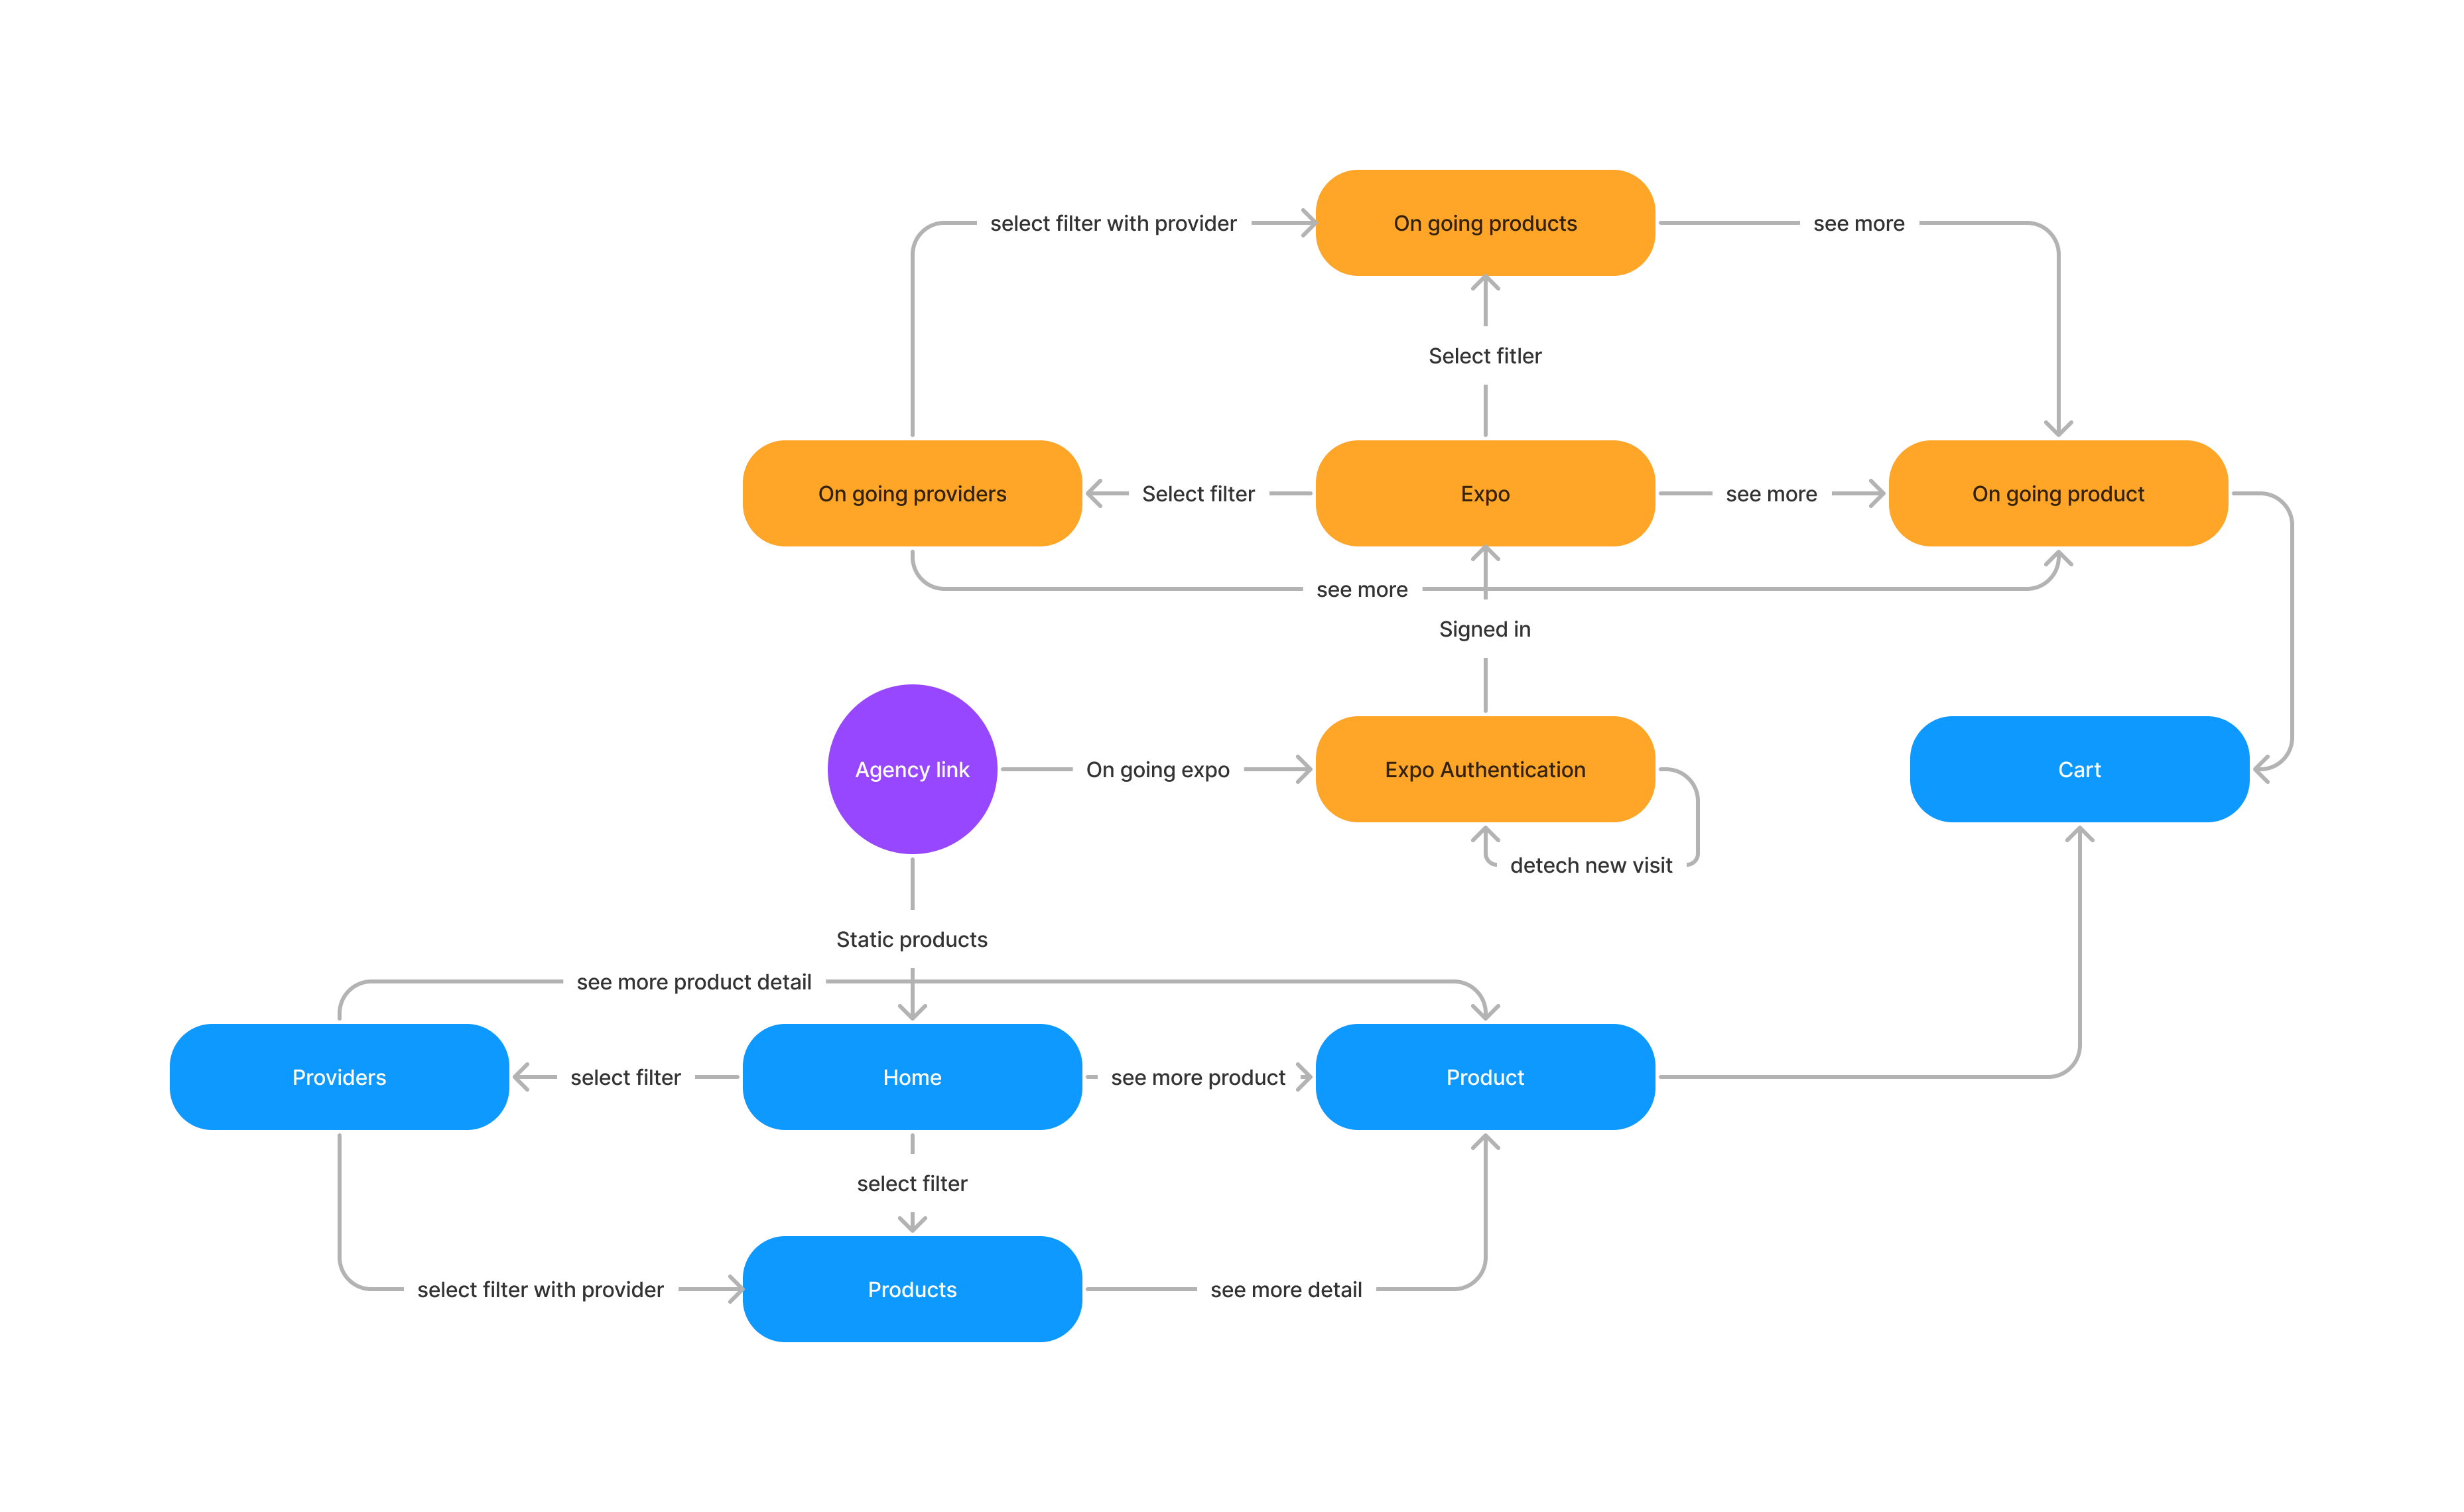
\includegraphics[width=\textwidth]{state.png}
	\label{fig:state}
\end{figure}
%
\section{Kết quả đạt được}

{\Huge fashion.ocopee.com}

\subsection{Dự án đã phát hành thực tế}

\subsubsection{Trạng thái ổn định}

shopwheydanang.com
mayberoom.vn
b21shoemaker.store
hypesneaker.vn
yensaodatquang.vn

\subsubsection{Chưa hoàn thiện, đang phát triển thêm}

japan-apple.jp
madeuniform.vn
khoailangtradoa.com
ocopee.com

\subsection{Dự án đang thử nghiệm}
fashion.ocopee.com

\section{Những vấn đề hạn chế}

\section{Hướng phát triển}
